\chapter{CRM ehnance by Artificial Intelligence}
\label{sec:crm-ai}


% -------------------------------- Section: What is a CRM
\section{Customer Relationship Management}

% What is a CRM
With a total market revenue of \$39.5 billion in 2017 and an expected growth rate of 16\% for 2018, Customer Relationship Management (CRM) became largest segment of enterprise applications\cite{gartner-crm-market}. From it most basic form as an \textit{Excel} spreadsheet to a more complete cloud-based solution, a CRM is an approach for managing the organization's relationships and interactions with current and potential customers alongside with the data and information associated to them\cite{salesforce:CRM-def}.

% Why is it useful
There are many possible descriptions for customer relationship management. At high-level, it as a transversal organizational strategy that allows a company to better understand, anticipate and manage the needs of current and potential customers by placing them at the heart of the system\cite{brown2000customer}\nocite{biedermann-crm}. A CRM is a complete set of tools to follow, understand, and nurture all interactions between a company and its customers. It supports the relationship through the entire customer life-cycle, from the prospects to loyal customers. 

CRM systems aim to maintain a good relationship with customers, which leads to revenues for the company. Indeed, some studies point out that managing long-term relationships with clients is worth the effort, as it is five times more expensive to acquire new customers than to keep current ones\cite{crm-facts}. Developing and focusing solely on products is not an option for companies, because bad user experience will hurt the business in the long-term\footnote{It's reported that one unsatisfied customer talks to 12 other customers while one satisfied talk to four customers. Businesses must be willing to sacrifice short term advantage for long term gains \cite{crm-facts,bennet,crm-essay}}.

% What a CRM does
An important aspect of CRM systems are their ability to store and share data. From the first contact with customer until the last question asked to the customer service, this data can be shared across all departments within the company. It avoids data silos and incomplete information and enables to gain a 360° vision of the customer relationship with all touchpoints inside the company \cite{efficy-crm}.

A CRM can also be viewed as a set of macro-level process that subsumes numerous sub-processes\cite{crm-processes}. These processes must be aligned between the business's needs and IT operations. As shown in figure \ref{fig:crm-clc}, these functional processes support the entire customer life cycle.

\begin{figure}[h]
    \centering
    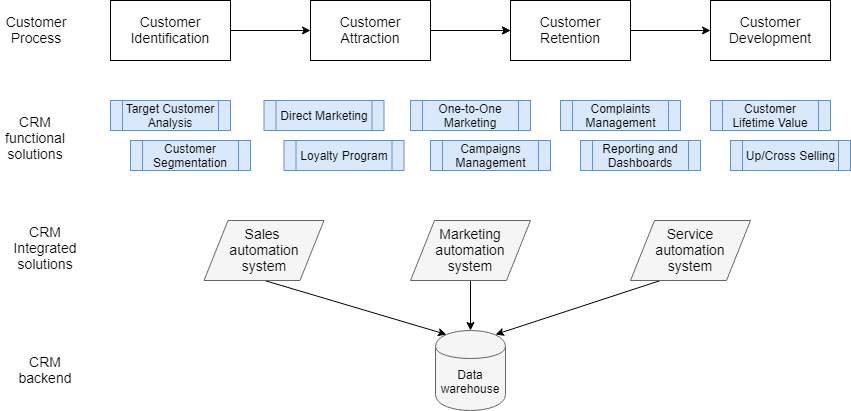
\includegraphics[width=12cm]{images/CRM-CustomerLifeCycle.png}
    \caption[CRM supports the customer life cycle]{CRM supports the customer life cycle. From \cite{DataAnalyticsinCRMProcessesALiteratureReview}}
    \label{fig:crm-clc}
\end{figure}

% How it does it
CRM systems are usually organized around four axes: Sales, Marketing, Support and Analysis\cite{crm-def}. The first three concern the operational part of a CRM, used for lead generation and conversion for example. An analytical part of the CRM takes care to analyze and generate insights from the data generated and collected by the operational processes. Through the years, CRM systems produce and store more and more data and \textit{Big data} techniques are needed used to make use of them, instead of just having them stored\cite{peel-et-al}.


% -------------------------------- Section: Why AI within CRM
\section{CRM AI}

CRM AI is a term that can be found in the litterature. But what does it really means ? Is it more than just a buzzword ? This section outlines the motivation and questions arising when combining CRM + AI.

This section details the motivations for combining CRM+AI and the resulting questions and interrogations.

\subsection{Artificial Intelligence within CRM}

Often cited as the next major vague of innovaiton, Artificial Intelligence (AI) can be the tool to optimize customer interactions based on the amount of data companies have. In its \textit{IT Glossary}\footnote{\url{https://www.gartner.com/it-glossary/artificial-intelligence/}}, Gartner defines AI as a technology that appears to emulate human performance. AI learns, comes to its own conclusion, appears to understand complex content, can engage into a natural dialogue with people, enhances human cognitive performance or replaces people in the execution of nonroutine tasks.

In a customer relationship management context, artificial intelligence can be used to enhance the current functionalities of CRMs. AI relies on data and for a company, all its customer-related data are stored in the CRM. By applying AI technologies into CRM applications like sales or service automation, current processes can evolve and new functionalities be created. AI has the ability to ingest data and assist CRM's user in their daily tasks, whether by intelligently analyzing a large volume of data or by being proactive and anticipating needs. The aim is to create more personalized customer experiences with findings uncovered by AI techniques and make a business \textit{smarter}


\subsection{Outline of the analysis}
% -------- Goal of the analysis
One of the aims of this thesis is to provided an overview of the integration of artificial intelligence technologies in a CRM context. With the advent of artificial intelligence and its relative ease of access, CRM vendors can consider a new product line around AI. When a CRM editor announces that it will soon integrate some AI components in its solutions, it aims to attract new customers while showing current customers that its system is innovative and at the cutting edge of technology.

CRM vendors claim to have easy to use and well integrated AI solutions, but what is offered in these solutions? What are the kind of AI technologies used? How easy to configure are those AI features? Are they really tailored and useful for the business? All companies are different, but can they adapt these innovative solutions to their unique business? What AI functionalities will become \textit{mandatory} for a good CRM? The research of this section tries to address those issues and really understand what is meant by \textit{CRM AI}.


% -------------------------------- Section: Editors Market
\section{Editors Market}


\subsection{CRM Editors analyzed}
The CRM software market is growing rapidly, especially due the awareness of customer experience's importance and the expansion of the cloud-based solutions\cite{crm-revenue}. Indeed, all types of companies, regardless of their size or revenues, can have their own CRM without the need to invest time and money in hardware. Opposed to on-premise deployment, where the CRM runs in the infrastructure created and maintained by the company, cloud-based deployment are today the most request deployment configuration\footnote{In 2008, only 12\% of the requests had a preference for cloud-based deployment. Six years later the trend is totally reversed, with 87\% of the deployment's requests regarding cloud-based solutions and 13\% on-premise CRMs \cite{crm-deployment-stats}.}.

There is a lot of offers in the CRM market\footnote{For example, \textit{Wikipedia} lists a total of 29 CRM systems.}. Some editors build complete CRM solution while smaller ones are only focus on one or two applications, like a sales force automation or customer engagement solutions. The editors analyzed in this project have been selected based on Gartner's \textit{Magic Quadrant}\footnote{Gartner is a research and advisory firm providing analysis on the information technology field.}. Two types of magic quadrant are directly related to customer relationship management: sales force automation and customer engagement center (figures \ref{fig:magic-quadrant-sales-force} and \ref{fig:magic-quadrant-customer-engagement}). A magic quadrant contains four groups to classify CRMs and in this research, all global CRMs classified as \textit{Leaders} are considered: \textit{Salesforce}, \textit{Microsoft}, \textit{Oracle} and \textit{Pegasystems}. Despite not being classified as a \textit{leader}, \textit{SAP} is also considered since it is the third largest publisher\cite{crm-market-share}. These five CRMS are the big fishes in the market (40.4\% of the market) and are the most likely to invest in AI features. Nevertheless, to stand out in the market, smaller companies specialize their products around a specific CRM's applications. To be as complete as possible, CRM editors \textit{SugarCRM}, \textit{Infor}, \textit{Zoho} and \textit{Zendesk} are also investigated.

\begin{figure}[!h]
    \begin{minipage}[c]{0.48\linewidth}
        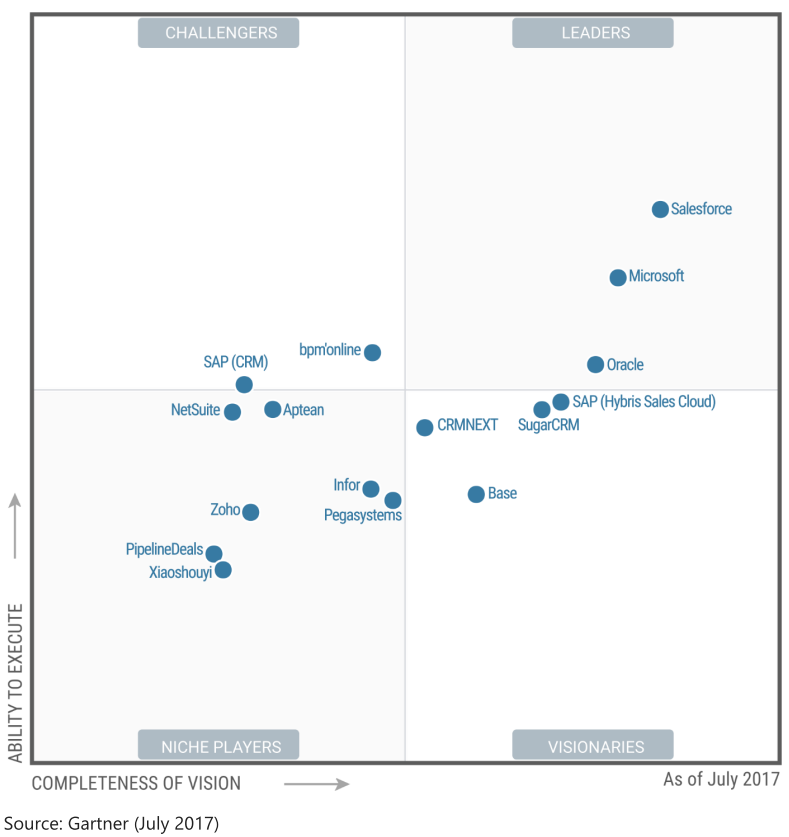
\includegraphics[width=\linewidth]{images/magic_quadrant_sales_force_automation.png}
        \caption[Magic Quadrant for Sales Force Automation]{Gartner, Magic Quadrant for Sales Force Automation, July 2017}
        \label{fig:magic-quadrant-sales-force}
    \end{minipage}
    \hfill
    \begin{minipage}[c]{0.49\linewidth}
        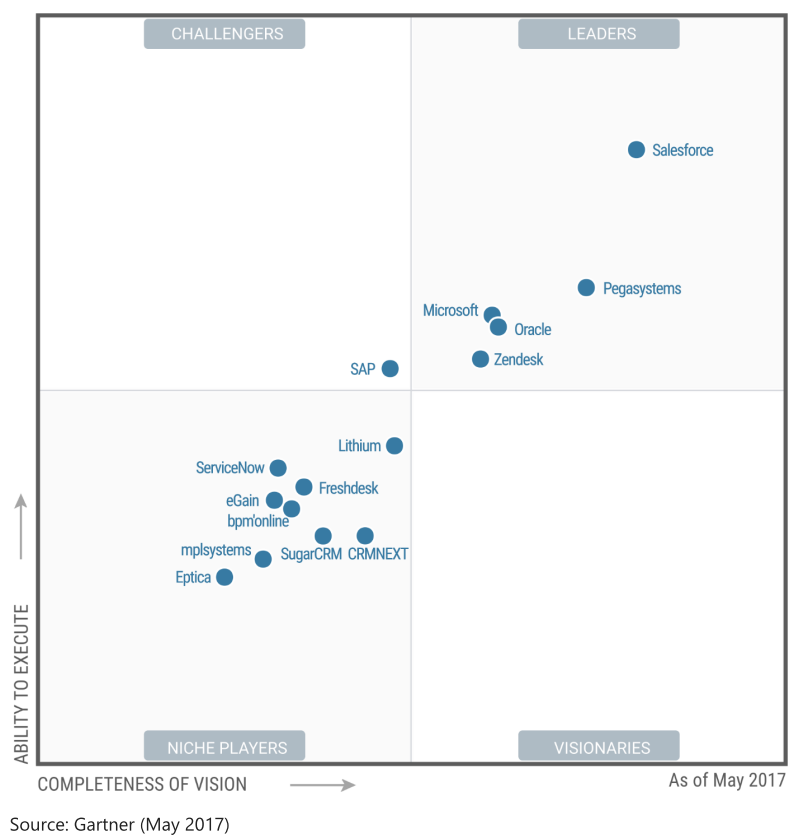
\includegraphics[width=\linewidth]{images/magic_quadrant_customer_engagement_center.png}
        \caption[Magic Quadrant for the CRM Customer Engagement Center]{Gartner, Magic Quadrant for the CRM Customer Engagement Center, May 2017}
        \label{fig:magic-quadrant-customer-engagement}
    \end{minipage}
\end{figure}

To analyze all those CRM editors, their website, press releases, community forums and knowledge base are used. Blog posts, specialized websites, and analyst firm's report are also widely used. Note that it wasn't possible to configure and test the functionalities detailed in the following sections. Products and features announced by CRM's editors after April 2018 are not taken into account in this research.

\subsection{CRM Editors review}

\subsubsection*{Dynamics 365}
Dynamics 365 is the customer relationhsip management product of Microsoft. Created in 2003 as Microsoft Dynamics CRM, the product was rebranded Dynamics 365 when an Enterprise Resource Planning (ERP) solution has been combined with the CRM. One of the key characteristics of Dynamics 365 is the native integration with other Microsoft products, like Microsoft Exchange, Office 365, Sharepoint and PowerBI. More recently, Dynamics 365 is building synergies with Azure technologies, which seems to be the foundation for AI inside Dynamics 365. 

Mid-2017 Microsoft launched the preview program of \textit{Dynamics Customer Insights}, a combined product of Azure and Dynamics 365 available through the Azure portal (and not built-in Dynamics 365). This product can support an entire machine learning project, from data collection to result's visualization. The data from Dynamics 365 can be combined with external data stored in \textit{csv} files under the same datamodel. The tool used Natural Language Processing (NLP) techniques to link the data from different sources together, based on a name, a street address or a phone number for example. The user can then select a variable (continuous number or boolean) and a predictive machine learning model will be generated, based on the data imported into \textit{Dynamics Customer Insights}. The model is probably a linear model generated with \textit{AutoML} techniques\footnote{Automated Machine Learning, abbreviated \textit{AutoML}, are algorithms to automatically select a good model, choose its hyperparameters, and perform features preprocessing steps for a new dataset. \cite{NIPS2015_5872}}. With the model generated, \textit{Dynamics Customer Insights} can use the predictions to create customer segments and visualization.

AI features directly built-in Dynamics 365 are not yet available, but Microsoft releases some preview features such as intelligent knowledge based articles suggestion to deal with customer's question in CRM's tickets and lead scoring. Lead scoring assigns a score for each lead or potential new customer based on the lead's profile and all previous leads stored in CRM's historical data.

\subsubsection*{Infor CRM}
Infor is a business cloud application provider that offers a CRM as part of its \textit{Customer Experience Suite}. Infor CRM - that's the name of the product - is composed of sales, marketing, and customer service applications. In July 2017, Infor announced \textit{Coleman}, an AI platform available as a virtual assistant. Accessible by voice or chat, CRM users use it to perform simple and predefined tasks, such as searching for information related to a CRM' contact or aggregating sales revenue for the last month. Infor CRM is available as a \textit{SaaS} hosted in \textit{Amazon Web Services} (AWS) and Coleman was built with \textit{Amazon Lex}, a product meant to build conversational interfaces. This seems to be Infor's strategy for AI: using existing frameworks such as AWS to extend their CRM functionalities.

Infor also claims to have a sales intelligence for CRM, with features that give insights about the next likely purchase of a customer, the customer's risk of churn and client segmentation based on their purchase history. It is not clear if those features are already implemented, as they only appear in Infor's marketing content.\nocite{infor-website}


\subsubsection*{Oracle}
Second-largest software maker by revenue after Microsoft, Oracle proposes CRM solutions via two products: \textit{Oracle Siebel} for on-premise deployments and \textit{Oracle CRM} for SaaS. Only available for the cloud, \textit{Adaptive Intelligence} applications have been launched in 2017. Instead of regrouping all their AI solutions under a general brand name, Oracle claims to \textit{avoid the hype and focusing on building apps that people can make money with}\cite{https://www.techemergence.com/crm-artificial-intelligence-trends-across-salesforce-oracle-sap/}. The philosophy is to build ready-to-use applications that CRM users can quickly integrate into their current system to add a layer of \textit{intelligence}.

These adaptive intelligent applications\footnote{\textit{Adaptive Intelligent} apps can also be abbreviated \textit{AI} apps...} announced by Oracle concern several areas of customer relationship management, from the sales - next best sales actions or lead scoring - to the customer service - automated answers - to the marketing division -  audiences segmentation, optimized campaign channel and send time. Despite having been in contact with Oracle's team, it was not possible to have a list of the applications already available or to have details about some features, like the \textit{next best sales actions} feature. It seems that artificial intelligence components to be integrated into Oracle CRM are at an early stage of development and not ready to be used by users. 


\subsubsection*{Pega CRM}
Pegasystems Inc. is a software company developing a CRM product based on their business process management (BPM) expertise. Pega CRM's revenue is highly dependent on its on-premise solution: \textit{SaaS} is estimated to represent only 8\% of the total revenue according to Gartner. This explains why Pegasystems is the only CRM's editor in this study to propose AI features for both on-premise and cloud deployments.

Artificial Intelligence solutions are divided into two products. There is a virtual assistant which pre-built integration into Facebook Messenger, Amazon Alex and a chat. This assistant has no functionalities or scenarios: it is meant as a development framework with out-of-the-box NLP and text analytics capabilities, such as intent and entity detection. CRM developers can then built their own scenarios and processes. The virtual assistant can also be integrated to treat incoming emails. Such \textit{email assistant} can analyze the content and redirect an email to the most appropriate person.

A second product available in Pega CRM is named \textit{Customer Decision Hub}, a centralized set of AI capabilities deployed across CRM applications. For the marketing, a recommender system is used to propose the most appropriate product to customers. The sales application contains a lead and opportunity scoring feature as well as a customer risk of churn evaluation. There are also two products that have been announced recently. First, an AI-coach for salespeople providing personalized advises and tips to under-performing sellers. Finally, an update on the \textit{Customer Decision Hub} will enable to build machine learning models and integrated them directly into CRM's processes. This tool is meant to build predicting models in a similar way as \textit{Dynamics Customer Insights} does, but the user can choose the type of machine learning model to use. Models are saved in the \textit{Predictive Model Markup Language} (PMML) language\footnote{PMML is an XML file format for predictive models that can be exchanged between different analytical applications. It can contain data transformations (pre- and post-processing) as well as one or more predictive models \cite{pmml}.}. This enables users to import their own models, nevertheless with some restrictions. Models can also be defined as an \textit{Adaptive analytics} model that will be retrained when new customer data is available.

\subsubsection*{Salesforce}
Created in 1999 with only cloud solutions, Salesforce is the worldwide leader regarding customer relationship management systems. Between 2015 and 2016, Salesforce acquired several AI start-ups to build a team of 150 data engineers. This strategy enable the company to launch Salesforce Einstein, an artificial intelligence solution spanning over all products of the CRM.

For the sales department of a company, Einstein offers lead an opportunity scoring to prioritize client's the most likely to convert and a forecasting feature to estimate the sales for each sales-agent. It also gives \textit{insights} about a contact like the its overall happiness, computed with sentiment analysis on emails received but also company-specific information based on the news (for example the share price falls on the stock market). Marketing's department can use Einstein to personalize mass-emailing with a product that specific customers are successive to buy, powered by recommender systems. The \textit{Email Engagement Prediction} feature predicts for each customer its likelihood to open an email or unsubscribe from the newsletters. These predictions can be integrated into \textit{marketing journeys} to address customers in a more personalized manner. Salesforce can classify incoming customer tickets with Einstein and has announced recommended response and intelligent routing for mid-2018.

All features mentioned above are configurable without any coding-skills, but Salesforce created \textit{MyEinstein} an API-based service with to build custom applications. As of March 2018, this tool was composed of beta versions for \textit{Einstein Bots} with entity, intent, and sentiment analysis and \textit{Einstein Prediction Builder} to build predictive models similar to Dynamics Customer Insights.

In addition to adding new functionalites to \textit{Einstein}, Saleforce has built two major partnership regarding AI: one is with \textit{Google Analytics} to create better customer segmentation and another one with \textit{IBM Watson} to improve Einstein's abilities regarding unstructured data and problem-solving tasks.

\subsubsection*{SAP}
The SAP company (Systeme, Anwendugne und Produkte in der Datenverarbeitung) sells enterprise software such as an ERP or CRM. SAP has two products for customer relationship management: SAP CRM 7.0 for on-premise needs and SAP Hybris Service Cloud for online deployment. Only the last one is concerned about AI features from \textit{SAP Leonardo}, the platform to integrate AI features across their cloud platform. The company claims that SAP Leonardo can be used for analytics, machine learning, big data, blockchain, and Internet of Things (IoT).

Regarding SAP Hybris, several products relying on AI have been annouced, such as \textit{SAP Hybris Customer Attribution} to segment customers based on game theory, \textit{SAP Resume Matching} to classify candidatures for the human resources using CRM, \textit{SAP Cash Application} to match payments received with open bills, or \textit{SAP Service Ticket Intelligence} to route customer service tickets to the appropriate agent, assign a priority score to each ticket and proposed knowledge based article to resolve it. These solutions are available out-of-the-box without any coding-skills required. SAP also offers SAP Leonardo Machine Learning to train out-of-the-box algorithms based on TensorFlow models. This product comes with some pre-built services such as image recognition (object classification, face recognition) and text analytics (topic detection, similarity scoring). 

SAP is investing a lot in the AI for business field with two products announced for mid-2018: \textit{SAP Leonardo Conversation AI Foundation} to build chatbot in the same manner as the Microfot bot framework and \textit{SAP Predictive Analytics} to build predictive machine learning models in the same manner as \textit{Dynamics for Customer Insights}, but for on-premise solutions.


\subsubsection*{SugarCRM}
SugarCRM is the most important CRM's editor relying on an open-source technology. Back in 2016, SugarCRM announced its plans regarding the usage of AI inside CRM. Two products were under investigation. The first was \textit{Candace}, an AI-powered intelligent agent to assist users in their daily tasks, such as setting up meetings, throwing reminders or monitoring social networks to spot client's dissatisfaction signs. Another announcement concerned the \textit{Sugar Intelligence Service} product to bring AI-features like lead and opportunity scoring or text sentiment analysis into the CRM. Since then, no evolution has been announced. By reading blog posts written by SugarCRM's head of corporate strategy, artificial intelligence features are not a priority and they are taking a \textit{wait and see} approach \cite{sugarcrm1,sugarcrm2}.

\subsubsection*{Zendesk}
Zendesk is not a global CRM, it has no sales force automation nor developed marketing product. Nevertheless, it is one of the leaders for customer support solutions, extremely popular in mid-size companies. Zendesk has a full range of AI functionalities regarding customer's tickets: redirection to the most appropriate person, automated prioritization, and customer risk of churn. It can compute a satisfaction prediction score for each customer, based on the ticket content and client's support history. Zendesk also offers a framework to develop chatbots.

\subsubsection*{ZohoCRM}
Zoho Corporation is specialized in developing business and IT solutions available as SaaS. The CRM - \textit{ZohoCRM} - has all its AI features regrouped under \textit{Zia}, described as an artificial intelligence powered sales assistant. Triggered by voice or chat, the Zia assistant performs some pre-defined tasks such as adding a note to a meeting or retrieving client's contact information. Zoho provides an user-interface to create new capabilities for Zia without any coding- skills required.

Zia is a chatbot but it also encapsulates other AI features of ZohoCRM, among which lead scoring, anomalies detection to control sales, email sentiment analysis and an indication on the best time to contact each client. It also proposes a feature to monitor the tasks perform by CRM's user and proactively suggest new processes for a better efficiency. It's not clear if artificial intelligence techniques are really being used for these functionalities. While it is obvious that email's sentiment analysis relies on NLP algorithms, the anomalies detection or best time to contact a client features can be done without any kind of AI. Those AI features are black-boxes to be used \textit{as-is} in the CRM.

% -------------------------------- Section: DMP Platforms
\section{Data Management Platforms}
May be just a subsection, very fast on the subject

--> ADOBE HERE ?


% -------------------------------- Section: Editors Ranking
\section{CRM Editors Ranking}
Speak about the roadmap here also

Specify that Einstein "explains" the Scores and motivation for prediction in lead scoring

\subsection{Current state}


\subsection{Near feature status}


% -------------------------------- Section: Conclusion
\section{Conclusion}

Gartner:

    - CRM editors are leveraging AI capabilities such as machine learning and NLP to augment their application functionality. The current work made by the CRM editors concern embedded AI.
    - The advantage for a company to use such embedded AI is the ability to use a powerful emerging technology quickly, without a lot of investments. 
    - This is the premise of using AI in CRM.
    - In the market, CRM editors are using AI as an umbrella term to encompass a wide array of functionality, including machine learning (ML) powered data predictions and natural-language processing (NLP) pseudohuman interactions (e.g. chatbots).  CRM editors are integrating such new functionalities within their applications to enhance their CRM functionality.


    - The integrated CRM AI capabilities offered by enterprise vendors provide a path to learn and experiment with ML and NLP services without needing deep AI-based technical skills.
    - Current embedded AI offerings apply advance data-driven predictive capabilities to optimize customer-related decisions against narrow CRM functional use-cases.
    - CRM Editors will continue to invest in incremental improvements. This will lead to increased customization, configuration, and transparency into the underlying technical execution process of their embedded AI capabilities.
    - Using AI CRM functionality will not make CRM users data scientist. However, packaged CRM AI capabilities provide a path tho learn and experiment ML and NLP technologies directly with real-world data.
    - Create more differentiated solutions by integrating custom-defined ML models into your CRM applications once you have identified the unique data patterns and possible insights that embedded fucntionality has not.
    - Black box implementations. API acess to pretrained AI.
    - Today’s AI in CRM aims to act as an assistant to human sales and marketing staffs. It can advise and point out opportunities and problems, but the judgment and action depends on the human.
    - Lead scoring, for example, is a fertile field for AI in CRM. The AI system can analyze a wealth of information about prospects and rank them according to their likelihood to purchase. The list can be presented to the sales staff with the most promising prospects first and the sales force can take it from there. A great application of CRM data is predicting activity. All sorts of events can be predicted using the historical data in the CRM database, including likelihood of making contact at a specific time of day and the probability of response to an email. A lot of the potential sales executives want to see is to predict the future so they can better plan.
    - Customer segmentation

    - Add the features ignored slide -> slide n°12